% Options for packages loaded elsewhere
\PassOptionsToPackage{unicode}{hyperref}
\PassOptionsToPackage{hyphens}{url}
%
\documentclass[
]{book}
\usepackage{lmodern}
\usepackage{amsmath}
\usepackage{ifxetex,ifluatex}
\ifnum 0\ifxetex 1\fi\ifluatex 1\fi=0 % if pdftex
  \usepackage[T1]{fontenc}
  \usepackage[utf8]{inputenc}
  \usepackage{textcomp} % provide euro and other symbols
  \usepackage{amssymb}
\else % if luatex or xetex
  \usepackage{unicode-math}
  \defaultfontfeatures{Scale=MatchLowercase}
  \defaultfontfeatures[\rmfamily]{Ligatures=TeX,Scale=1}
\fi
% Use upquote if available, for straight quotes in verbatim environments
\IfFileExists{upquote.sty}{\usepackage{upquote}}{}
\IfFileExists{microtype.sty}{% use microtype if available
  \usepackage[]{microtype}
  \UseMicrotypeSet[protrusion]{basicmath} % disable protrusion for tt fonts
}{}
\makeatletter
\@ifundefined{KOMAClassName}{% if non-KOMA class
  \IfFileExists{parskip.sty}{%
    \usepackage{parskip}
  }{% else
    \setlength{\parindent}{0pt}
    \setlength{\parskip}{6pt plus 2pt minus 1pt}}
}{% if KOMA class
  \KOMAoptions{parskip=half}}
\makeatother
\usepackage{xcolor}
\IfFileExists{xurl.sty}{\usepackage{xurl}}{} % add URL line breaks if available
\IfFileExists{bookmark.sty}{\usepackage{bookmark}}{\usepackage{hyperref}}
\hypersetup{
  pdftitle={Introduction to Quantitative Techniques in R for Conservation Biology},
  pdfauthor={Dr.~Yolanda Wiersma},
  hidelinks,
  pdfcreator={LaTeX via pandoc}}
\urlstyle{same} % disable monospaced font for URLs
\usepackage{color}
\usepackage{fancyvrb}
\newcommand{\VerbBar}{|}
\newcommand{\VERB}{\Verb[commandchars=\\\{\}]}
\DefineVerbatimEnvironment{Highlighting}{Verbatim}{commandchars=\\\{\}}
% Add ',fontsize=\small' for more characters per line
\usepackage{framed}
\definecolor{shadecolor}{RGB}{248,248,248}
\newenvironment{Shaded}{\begin{snugshade}}{\end{snugshade}}
\newcommand{\AlertTok}[1]{\textcolor[rgb]{0.94,0.16,0.16}{#1}}
\newcommand{\AnnotationTok}[1]{\textcolor[rgb]{0.56,0.35,0.01}{\textbf{\textit{#1}}}}
\newcommand{\AttributeTok}[1]{\textcolor[rgb]{0.77,0.63,0.00}{#1}}
\newcommand{\BaseNTok}[1]{\textcolor[rgb]{0.00,0.00,0.81}{#1}}
\newcommand{\BuiltInTok}[1]{#1}
\newcommand{\CharTok}[1]{\textcolor[rgb]{0.31,0.60,0.02}{#1}}
\newcommand{\CommentTok}[1]{\textcolor[rgb]{0.56,0.35,0.01}{\textit{#1}}}
\newcommand{\CommentVarTok}[1]{\textcolor[rgb]{0.56,0.35,0.01}{\textbf{\textit{#1}}}}
\newcommand{\ConstantTok}[1]{\textcolor[rgb]{0.00,0.00,0.00}{#1}}
\newcommand{\ControlFlowTok}[1]{\textcolor[rgb]{0.13,0.29,0.53}{\textbf{#1}}}
\newcommand{\DataTypeTok}[1]{\textcolor[rgb]{0.13,0.29,0.53}{#1}}
\newcommand{\DecValTok}[1]{\textcolor[rgb]{0.00,0.00,0.81}{#1}}
\newcommand{\DocumentationTok}[1]{\textcolor[rgb]{0.56,0.35,0.01}{\textbf{\textit{#1}}}}
\newcommand{\ErrorTok}[1]{\textcolor[rgb]{0.64,0.00,0.00}{\textbf{#1}}}
\newcommand{\ExtensionTok}[1]{#1}
\newcommand{\FloatTok}[1]{\textcolor[rgb]{0.00,0.00,0.81}{#1}}
\newcommand{\FunctionTok}[1]{\textcolor[rgb]{0.00,0.00,0.00}{#1}}
\newcommand{\ImportTok}[1]{#1}
\newcommand{\InformationTok}[1]{\textcolor[rgb]{0.56,0.35,0.01}{\textbf{\textit{#1}}}}
\newcommand{\KeywordTok}[1]{\textcolor[rgb]{0.13,0.29,0.53}{\textbf{#1}}}
\newcommand{\NormalTok}[1]{#1}
\newcommand{\OperatorTok}[1]{\textcolor[rgb]{0.81,0.36,0.00}{\textbf{#1}}}
\newcommand{\OtherTok}[1]{\textcolor[rgb]{0.56,0.35,0.01}{#1}}
\newcommand{\PreprocessorTok}[1]{\textcolor[rgb]{0.56,0.35,0.01}{\textit{#1}}}
\newcommand{\RegionMarkerTok}[1]{#1}
\newcommand{\SpecialCharTok}[1]{\textcolor[rgb]{0.00,0.00,0.00}{#1}}
\newcommand{\SpecialStringTok}[1]{\textcolor[rgb]{0.31,0.60,0.02}{#1}}
\newcommand{\StringTok}[1]{\textcolor[rgb]{0.31,0.60,0.02}{#1}}
\newcommand{\VariableTok}[1]{\textcolor[rgb]{0.00,0.00,0.00}{#1}}
\newcommand{\VerbatimStringTok}[1]{\textcolor[rgb]{0.31,0.60,0.02}{#1}}
\newcommand{\WarningTok}[1]{\textcolor[rgb]{0.56,0.35,0.01}{\textbf{\textit{#1}}}}
\usepackage{longtable,booktabs}
\usepackage{calc} % for calculating minipage widths
% Correct order of tables after \paragraph or \subparagraph
\usepackage{etoolbox}
\makeatletter
\patchcmd\longtable{\par}{\if@noskipsec\mbox{}\fi\par}{}{}
\makeatother
% Allow footnotes in longtable head/foot
\IfFileExists{footnotehyper.sty}{\usepackage{footnotehyper}}{\usepackage{footnote}}
\makesavenoteenv{longtable}
\usepackage{graphicx}
\makeatletter
\def\maxwidth{\ifdim\Gin@nat@width>\linewidth\linewidth\else\Gin@nat@width\fi}
\def\maxheight{\ifdim\Gin@nat@height>\textheight\textheight\else\Gin@nat@height\fi}
\makeatother
% Scale images if necessary, so that they will not overflow the page
% margins by default, and it is still possible to overwrite the defaults
% using explicit options in \includegraphics[width, height, ...]{}
\setkeys{Gin}{width=\maxwidth,height=\maxheight,keepaspectratio}
% Set default figure placement to htbp
\makeatletter
\def\fps@figure{htbp}
\makeatother
\setlength{\emergencystretch}{3em} % prevent overfull lines
\providecommand{\tightlist}{%
  \setlength{\itemsep}{0pt}\setlength{\parskip}{0pt}}
\setcounter{secnumdepth}{5}
\usepackage{booktabs}
\usepackage{amsthm}
\makeatletter
\def\thm@space@setup{%
  \thm@preskip=8pt plus 2pt minus 4pt
  \thm@postskip=\thm@preskip
}
\makeatother
\ifluatex
  \usepackage{selnolig}  % disable illegal ligatures
\fi
\usepackage[]{natbib}
\bibliographystyle{apalike}

\title{Introduction to Quantitative Techniques in R for Conservation Biology}
\author{Dr.~Yolanda Wiersma}
\date{2021-02-17}

\begin{document}
\maketitle

{
\setcounter{tocdepth}{1}
\tableofcontents
}
\hypertarget{introduction}{%
\chapter{Introduction}\label{introduction}}

Biology, including ecology and conservation, is becoming increasingly quantitative. Familiarity with a range of statistical tools (frequentist, multivariate, Bayesian) is expected. Many researchers draw on quantitative methods; whether it is process or mathematical modelling, programming, bioinformatics, or bioeconomic analyses. We will only touch on key concepts in quantitative methods; in-depth training would require multiple full-semester courses.

In the process of increasing quantitative skills across the Biology curriculum, we have prepared an online guide for using R, that is designed for new users, and as a reference document for all Biology students. You can access it \href{https://ahurford.github.io/quant-guide-all-courses/}{here}.
In this three-week module, we will carry out a few exercise that mimics some of the quantitative skills that you need to be a successful conservation biologist. These include:

\begin{enumerate}
\def\labelenumi{\arabic{enumi}.}
\tightlist
\item
  Data management (with an introduction to the \texttt{dplyr} package)
\item
  Plotting data effectively (with an introduction to the \texttt{ggplot2} package)
\item
  Univariate and multivariate statistical analysis (with an introduction to the \texttt{vegan} package)
\end{enumerate}

\hypertarget{data}{%
\chapter{Data for this manual}\label{data}}

We are using three data sets from the Mid-Atlantic Coastal Plain (MACP). An analysis with these data is described in a paper by \citet{McMullin2019}. The data sets are available as CSV files on Brightspace and are as described briefly below.

\begin{itemize}
\item
  MACPsites.csv: a database of site attributes (215 rows; 1 row per site). Attributes are coded as

  \begin{itemize}
  \tightlist
  \item
    ER: Ecoregion name
  \item
    VEG: Vegetation type
  \item
    PPT: Average annual precipitation (in mm)
  \item
    TEMP: Average annual temperature (in degrees Celsius)
  \item
    ELEV: Elevation above sea level (in m)
  \end{itemize}
\item
  MACPspp.csv: a species by site matrix. Sites are in rows (215 rows; 1 row per site) and species are columns (599). Full names of species associated with each code are in the Supplemental material to the \citet{McMullin2019} paper.
\item
  MACPtraits.csv: a species by traits matrix. Species are rows (599 rows; 1 row per species) with 4 columns of trait categories. Traits are

  \begin{itemize}
  \tightlist
  \item
    Photobiont: indicates which algae or cyanobacteria is the photobiont partner for that lichen
  \item
    Reproductive.Mode: indicates how the lichen reproduceds
  \item
    Reproductive.Structure: indicates what kind of reprodcutive structure(s) that species has
  \item
    Substrate: indicates what kind of substrate this species is usually found on
  \end{itemize}
\end{itemize}

\hypertarget{part-1.-data-wrangling-datamgmt}{%
\chapter{Part 1. Data Wrangling (\#dataMgmt)}\label{part-1.-data-wrangling-datamgmt}}

This section teaches some tricks and tips for data wrangling using the \texttt{dplyr} package. It reviews some of the more detailed introduction to \texttt{dplyr} from BIOL 1002 labs. If you would like to review the lab manual for BIOL 1002, you can access it \href{https://jakep962.github.io/Biol_1002/index.html}{here}.

A useful ``cheatsheet'' to print out and hang by your desk for this module is the \texttt{dplyr} \href{https://rstudio.com/wp-content/uploads/2015/02/data-wrangling-cheatsheet.pdf}{cheatsheet}

\hypertarget{step-1---install-package-and-read-in-files}{%
\section{Step 1 - Install package and read in files}\label{step-1---install-package-and-read-in-files}}

\begin{itemize}
\tightlist
\item
  install and load the package \texttt{dplyr} (if you don't remember how to do this, refer to Section 4.10 of the \href{https://ahurford.github.io/quant-guide-all-courses/rintro.html\#r-packages}{Biology R Guide}
\end{itemize}

\begin{verbatim}
## 
## Attaching package: 'dplyr'
\end{verbatim}

\begin{verbatim}
## The following objects are masked from 'package:stats':
## 
##     filter, lag
\end{verbatim}

\begin{verbatim}
## The following objects are masked from 'package:base':
## 
##     intersect, setdiff, setequal, union
\end{verbatim}

\begin{itemize}
\tightlist
\item
  read in the three data sets. The code is given below, you can chose to give the dataframes different names, but for ease of following along it would be wise to use the same as here.
\end{itemize}

\begin{Shaded}
\begin{Highlighting}[]
\NormalTok{MACPsites }\OtherTok{\textless{}{-}} \FunctionTok{read.csv}\NormalTok{(}\StringTok{"MACPsites.csv"}\NormalTok{)}
\NormalTok{MACPspp }\OtherTok{\textless{}{-}} \FunctionTok{read.csv}\NormalTok{(}\StringTok{"MACPspp.csv"}\NormalTok{)}
\NormalTok{MACPtraits }\OtherTok{\textless{}{-}} \FunctionTok{read.csv}\NormalTok{(}\StringTok{"MACPtraits.csv"}\NormalTok{)}
\end{Highlighting}
\end{Shaded}

\hypertarget{step-2-create-a-new-column-and-add-it-to-a-dataframe}{%
\section{Step 2: Create a new column and add it to a dataframe}\label{step-2-create-a-new-column-and-add-it-to-a-dataframe}}

Use the \texttt{mutate} function in \texttt{dplyr} to create a column which sums all the species at that site, and writie it to a new dataframe called MACPspp\_sum. Note that this is a row-wise function and that I am using the \texttt{pipes} tool (denoted by the \texttt{\%\textgreater{}\%} symbol). If you would like to review using pipes, see Section 2.1.5 of the manual for \href{https://jakep962.github.io/Biol_1002/week1.html\#lab1}{BIOL1002}.

\begin{Shaded}
\begin{Highlighting}[]
\NormalTok{MACPspp\_sum }\OtherTok{\textless{}{-}}\NormalTok{ MACPspp }\SpecialCharTok{\%\textgreater{}\%}
  \FunctionTok{rowwise}\NormalTok{() }\SpecialCharTok{\%\textgreater{}\%}
  \FunctionTok{mutate}\NormalTok{(}\AttributeTok{sppRich =} \FunctionTok{sum}\NormalTok{(}\FunctionTok{c\_across}\NormalTok{(ABRhyp}\SpecialCharTok{:}\NormalTok{XYLnig)))}
\end{Highlighting}
\end{Shaded}

\hypertarget{step-3-querying-and-filtering-the-data}{%
\section{Step 3: Querying and filtering the data}\label{step-3-querying-and-filtering-the-data}}

Use the \texttt{filter} function in \texttt{dplyr} to select only those sites that have more than 80 species and use this to create a new dataframe called MACPhotspots. Check Section 2.1.1 of the Manual for \href{https://jakep962.github.io/Biol_1002/week1.html\#lab1}{BIOL1002} to review the code.

\textbf{HAND IN} Then try using a function to find out what the highest species richness is across all sites (\textbf{HINT} another word for highest richness is ``max``` richness). Describe what function you used (a code snippet would be fine!)

\begin{verbatim}
## [1] 142
\end{verbatim}

\hypertarget{step-4.-grouping-and-joining-data}{%
\section{Step 4. Grouping and Joining Data}\label{step-4.-grouping-and-joining-data}}

Because both the MACPsites data and the MACPspp data are arranged in rows, with one row per site, we can combine them into one dataframe that contains both the species and the environment data. We can do it like this:

\begin{Shaded}
\begin{Highlighting}[]
\NormalTok{MACPall }\OtherTok{\textless{}{-}} \FunctionTok{inner\_join}\NormalTok{(MACPsites, MACPspp\_sum, }\AttributeTok{by =} \StringTok{"site"}\NormalTok{)}
\end{Highlighting}
\end{Shaded}

\textbf{HAND IN}: How would you confirm that you have done this correctly (there are different ways)?

Sometimes we might want to group and summarize the data in different ways. For example, we might want to group the data by Ecoregion and then see what the mean richness is per ecoregion, to see if some ecoregions have higher richness than others. In the next section we will use these summary data to make some graphs.

\begin{Shaded}
\begin{Highlighting}[]
\NormalTok{EcoR\_spp }\OtherTok{\textless{}{-}} \FunctionTok{group\_by}\NormalTok{(MACPall, ER)}

\NormalTok{EcoR\_spp\_mean }\OtherTok{\textless{}{-}} \FunctionTok{summarize}\NormalTok{(EcoR\_spp, }\AttributeTok{mean\_rich =} \FunctionTok{mean}\NormalTok{(sppRich))}
\NormalTok{EcoR\_spp\_se }\OtherTok{\textless{}{-}} \FunctionTok{summarize}\NormalTok{(EcoR\_spp, }\AttributeTok{se\_rich =} \FunctionTok{sd}\NormalTok{(sppRich))}
\end{Highlighting}
\end{Shaded}

\hypertarget{what-to-hand-in-for-part-1.}{%
\chapter{What to hand in for Part 1.}\label{what-to-hand-in-for-part-1.}}

Summarize the results from above where it says \textbf{HAND IN}. As well, in one or two sentences explain the difference between the \texttt{select} , \texttt{filter} and \texttt{mutate} functions in the package \texttt{dplyr}.

\hypertarget{part-2.-making-effective-graphs-graphs}{%
\chapter{Part 2. Making Effective Graphs (\#graphs)}\label{part-2.-making-effective-graphs-graphs}}

In this section, we will make a few different types of graphs, using the package \texttt{ggplot2}. You'll also spend some time thinking about the best way to visualize different types of data.

You will need to install and load the package \texttt{ggplot2} and you might want to keep the ggplot2 \href{https://rstudio.com/wp-content/uploads/2016/11/ggplot2-cheatsheet-2.1.pdf}{cheatsheet} handy.

We'll start by making a simple barplot of mean species richness using the dataframes we created at the end of \citet{ref}(dataMgmt). The package ggplot works with datafames and not vectors (as is the case when using the \texttt{plot} function in \texttt{baseR}). The syntax of ggplot is also very elegant in that you can ``layer'' on data and themes to an existing plot using the \texttt{+} symbol at the end of each line -- we made use of this when we employed \texttt{ggplot2} to do GIS-type mapping in the previous \href{https://nlboreal.github.io/ConservationGIS/}{Module} for this course).

\begin{Shaded}
\begin{Highlighting}[]
\FunctionTok{ggplot}\NormalTok{(}\AttributeTok{data =}\NormalTok{ EcoR\_spp\_mean) }\SpecialCharTok{+}
  \FunctionTok{geom\_col}\NormalTok{(}\AttributeTok{mapping=} \FunctionTok{aes}\NormalTok{(}\AttributeTok{x =}\NormalTok{ ER, }\AttributeTok{y =}\NormalTok{ mean\_rich))}
\end{Highlighting}
\end{Shaded}

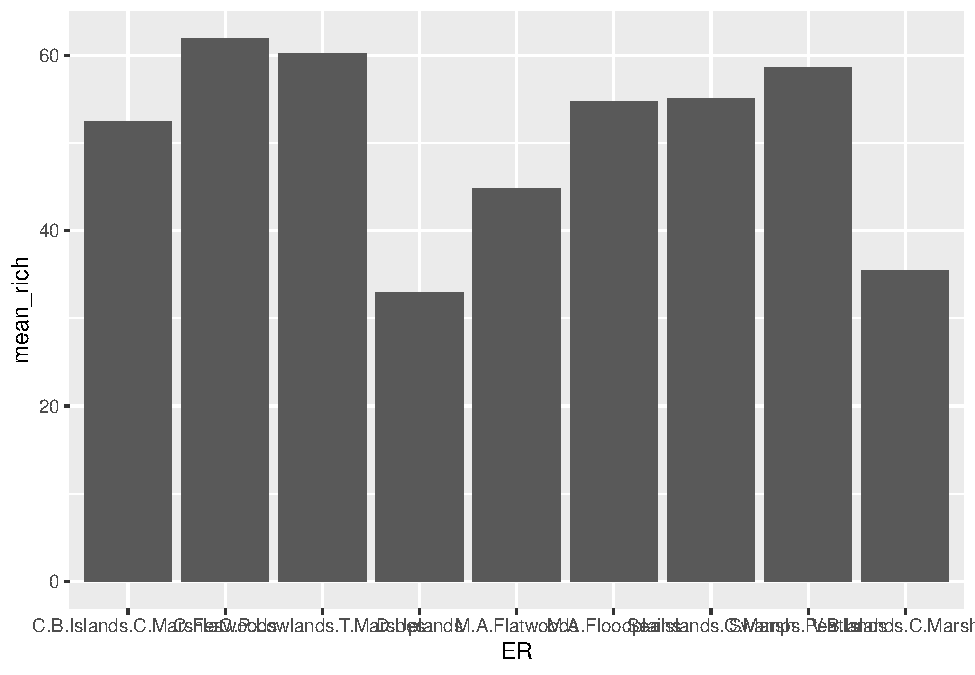
\includegraphics{bookdown-demo_files/figure-latex/unnamed-chunk-9-1.pdf}

You might notice that the text labels on the X-axis are not well-placed. We can adjust this by adding a \texttt{theme} that specifies the angle at which to display the text. Note that the first two lines of the code chunk below are identical to the chunk above, but with the \texttt{+} sign added at the end, so that we can add a line of code to add a \texttt{theme} function.

\begin{Shaded}
\begin{Highlighting}[]
\FunctionTok{ggplot}\NormalTok{(}\AttributeTok{data =}\NormalTok{ EcoR\_spp\_mean) }\SpecialCharTok{+}
  \FunctionTok{geom\_col}\NormalTok{(}\AttributeTok{mapping=} \FunctionTok{aes}\NormalTok{(}\AttributeTok{x =}\NormalTok{ ER, }\AttributeTok{y =}\NormalTok{ mean\_rich)) }\SpecialCharTok{+}
  \FunctionTok{theme}\NormalTok{(}\AttributeTok{axis.text.x =} \FunctionTok{element\_text}\NormalTok{(}\AttributeTok{angle =} \DecValTok{90}\NormalTok{))}
\end{Highlighting}
\end{Shaded}

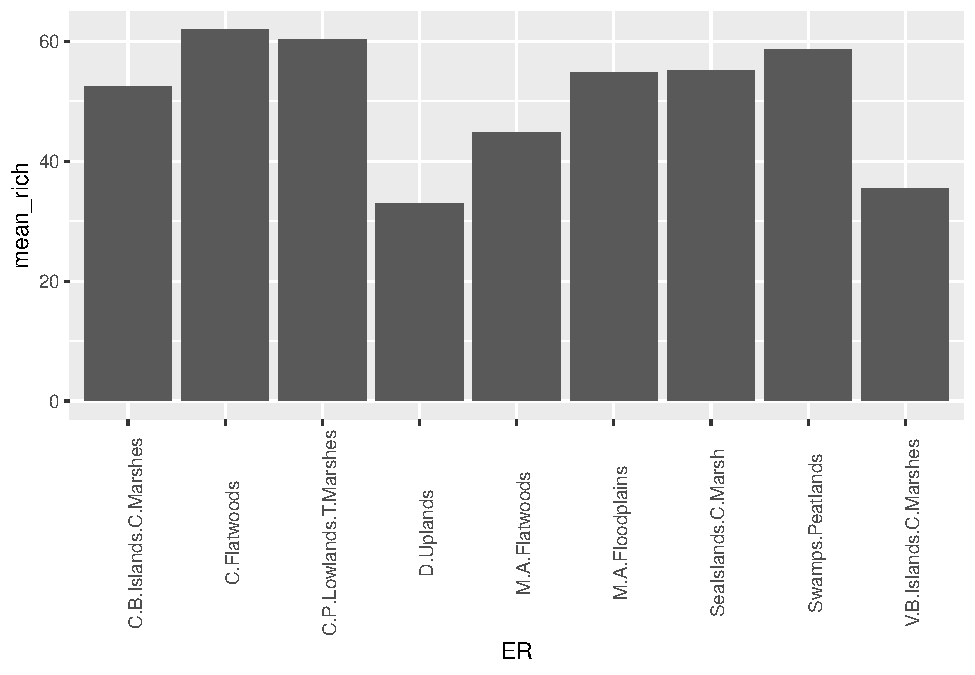
\includegraphics{bookdown-demo_files/figure-latex/unnamed-chunk-10-1.pdf}

To add error bars, one way we could do that is to first add the standard error we calculated in \citet{ref}(dataMgmt) to the dataframe that \texttt{ggplot2} is using, again using a \texttt{dplyr} function.

\begin{Shaded}
\begin{Highlighting}[]
\NormalTok{EcoR\_spp\_meanse }\OtherTok{\textless{}{-}} \FunctionTok{inner\_join}\NormalTok{(EcoR\_spp\_mean, EcoR\_spp\_se, }\StringTok{"ER"}\NormalTok{)}
\end{Highlighting}
\end{Shaded}

Then we simply add another \texttt{geom} function to the code snippet above, and adjust the \texttt{data\ =} code to reflect the new set with the standard error column added.

\begin{Shaded}
\begin{Highlighting}[]
\FunctionTok{ggplot}\NormalTok{(}\AttributeTok{data =}\NormalTok{ EcoR\_spp\_meanse) }\SpecialCharTok{+}
  \FunctionTok{geom\_col}\NormalTok{(}\AttributeTok{mapping=} \FunctionTok{aes}\NormalTok{(}\AttributeTok{x =}\NormalTok{ ER, }\AttributeTok{y =}\NormalTok{ mean\_rich)) }\SpecialCharTok{+}
  \FunctionTok{geom\_errorbar}\NormalTok{(}\AttributeTok{mapping =} \FunctionTok{aes}\NormalTok{(}\AttributeTok{x =}\NormalTok{ ER, }\AttributeTok{ymin =}\NormalTok{ mean\_rich, }\AttributeTok{ymax =}\NormalTok{ mean\_rich }\SpecialCharTok{+}\NormalTok{ se\_rich)) }\SpecialCharTok{+} 
  \FunctionTok{theme}\NormalTok{(}\AttributeTok{axis.text.x =} \FunctionTok{element\_text}\NormalTok{(}\AttributeTok{angle =} \DecValTok{90}\NormalTok{))}
\end{Highlighting}
\end{Shaded}

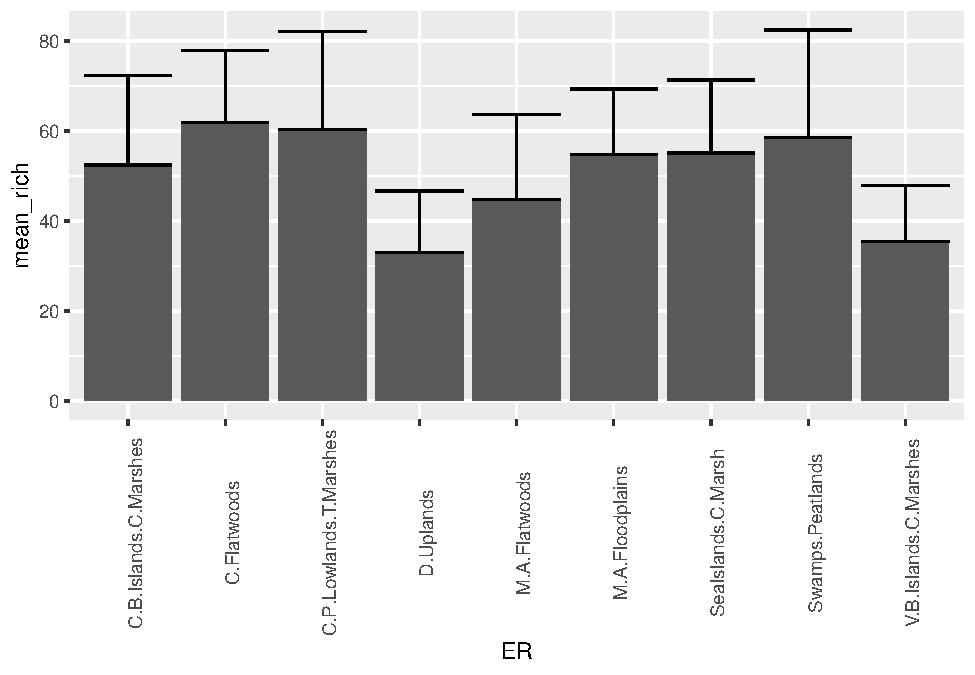
\includegraphics{bookdown-demo_files/figure-latex/unnamed-chunk-12-1.pdf}

\hypertarget{your-assignment-for-part-2}{%
\chapter{Your assignment for Part 2}\label{your-assignment-for-part-2}}

\begin{enumerate}
\def\labelenumi{\arabic{enumi}.}
\item
  Pick two variables in one of the datasets we're using here that would be best shown as a scatterplot. Feel free to join or group data from any of the 3 datasets to pracitse your data wrangling skills. Try adjusting the symbology and axis labels for maximum effect. Hand in a copy of your code and the finished figure. Justify why a scatterplot is an appropriate way to display these data.
\item
  \textbf{For graduate students (and ambitious undergrads)} In addition to the above step, pick a graph type in \texttt{ggplot2} that you have never created before (but that perhaps is a way you may want to visualize your own data for your graduate work), and pick the appropriate data from one or more of the sets avaialable here to create a figure. Hand in a copy of your code and the finished figure. Justify why the data chosen fit this kind of figure well.
\end{enumerate}

\hypertarget{part-3.-statistical-analysis-stats}{%
\chapter{Part 3. Statistical Analysis (\#stats)}\label{part-3.-statistical-analysis-stats}}

You will need to install and load package \texttt{vegan}.

\begin{verbatim}
## Loading required package: permute
\end{verbatim}

\begin{verbatim}
## Loading required package: lattice
\end{verbatim}

\begin{verbatim}
## This is vegan 2.5-7
\end{verbatim}

\hypertarget{univariate-analysis}{%
\section{Univariate Analysis}\label{univariate-analysis}}

We will be doing a simple Generalized Linear Model (GLM). You could easily do an entire course on GLMs, so this is not even going to begin to scratch the surface of what there is to learn about this type of statistical analysis.

In the paper by \citet{McMullin2019}, the authors examined which lichen sites and species might be most threatened by sea level rise. They did not look for other patterns of species distribution. Here we will test whether lichen richness follows the pattern predicted by the latitudinal species gradient that has been observed for other species.

Here is the code to create a GLM called \texttt{lat\_test} (short for ``latitude test''). We're simply testing whether latitude (``Lat'') explains species richness with a linear function.

\begin{Shaded}
\begin{Highlighting}[]
\NormalTok{lat\_test }\OtherTok{\textless{}{-}} \FunctionTok{glm}\NormalTok{(sppRich }\SpecialCharTok{\textasciitilde{}}\NormalTok{ Lat, }\AttributeTok{data =}\NormalTok{ MACPall)}
\end{Highlighting}
\end{Shaded}

To see the model output, type \texttt{summary(lat\_test)}.

It's always important to check that your model doesn't violate assumptions of normality. You can assess this by inspecting the ratio of the null deviance to residual deviance in the model summary.

You can do this by plotting the model fits. Do this with the code \texttt{plot(lat\_test)}. You will see plots of 1) residuals vs.~fitted data; 2) a Q-Q plot; 3) Scale-location plot; 4) Residuals vs.~Leverage.

Click the links here to read about how to interpret the \href{https://stats.stackexchange.com/questions/76226/interpreting-the-residuals-vs-fitted-values-plot-for-verifying-the-assumptions}{Residuals vs Fitted plot}; the \href{https://stats.stackexchange.com/questions/101274/how-to-interpret-a-qq-plot}{Q-Q plot}. If your model does not meet the assumptions of normality, you may need to use a different error structure (e.g., Poisson, logNormal). Going into the whys and hows of that is beyond the scope of this course. The Q-Q plot fit here for \texttt{lat\_test} is slightly skewed but we're going to accept it.

To make a scatterplot of the data with the line of best fit included, use the code below. Note the new function \texttt{predict.glm} which calls the model we built (\texttt{lat-test}) and builds a predictive line across the range of x-values in our plot. The code chunk below also demonstrates how to add customized x and y axis labels (third ``layer'' in the ggplot2 code). In the first line (\texttt{geom\_point} function), there is a demonstration of how to colour code the points by one of the attributes in the data base (in this case \texttt{ER} for Ecoregion) AND how to use \texttt{position=jitter} to add some slight noise to the data that allows you to see more points by minimizing overlap between points. This makes your graph slightly less accurate on a very fine scale, but enables you to see broader scale patterns. Both of these can be very useful functions.

\begin{Shaded}
\begin{Highlighting}[]
\FunctionTok{ggplot}\NormalTok{(}\AttributeTok{data =}\NormalTok{ MACPall) }\SpecialCharTok{+}
  \FunctionTok{geom\_point}\NormalTok{(}\AttributeTok{mapping =} \FunctionTok{aes}\NormalTok{(}\AttributeTok{x =}\NormalTok{ Lat, }\AttributeTok{y =}\NormalTok{ sppRich, }\AttributeTok{colour =}\NormalTok{ ER), }\AttributeTok{position =} \StringTok{"jitter"}\NormalTok{) }\SpecialCharTok{+}
  \FunctionTok{geom\_line}\NormalTok{(}\AttributeTok{mapping =} \FunctionTok{aes}\NormalTok{(}\AttributeTok{x =}\NormalTok{ Lat, }\AttributeTok{y =} \FunctionTok{predict.glm}\NormalTok{(lat\_test)), }\AttributeTok{size =} \DecValTok{1}\NormalTok{) }\SpecialCharTok{+}
  \FunctionTok{labs}\NormalTok{(}\AttributeTok{x =} \StringTok{"latitude"}\NormalTok{, }\AttributeTok{y =} \StringTok{"lichen species richness"}\NormalTok{)}
\end{Highlighting}
\end{Shaded}

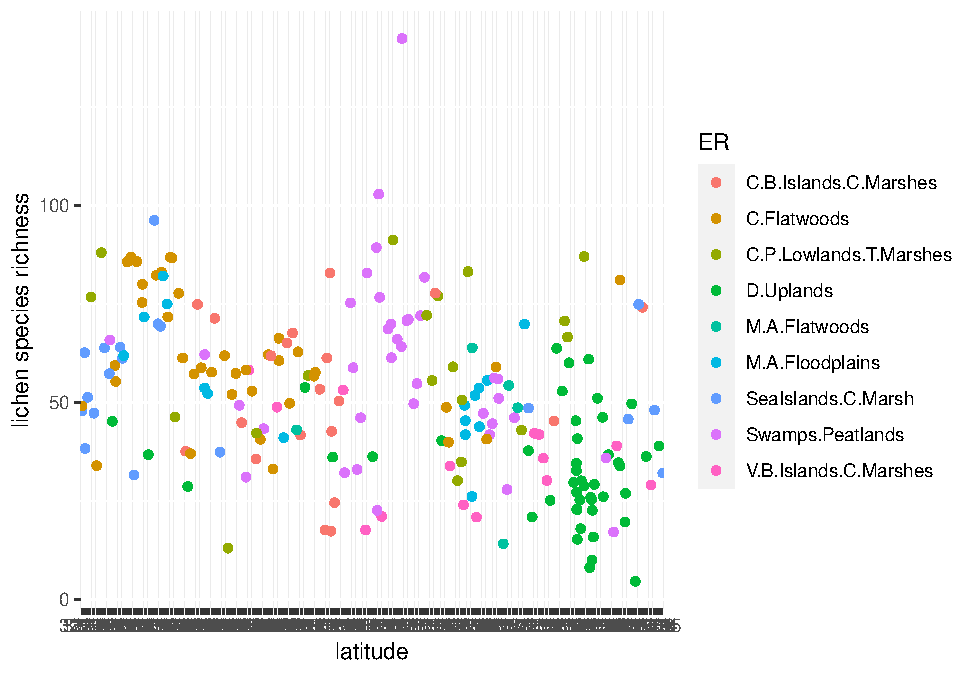
\includegraphics{bookdown-demo_files/figure-latex/unnamed-chunk-15-1.pdf}

\hypertarget{multivariate-analysis}{%
\section{Multivariate Analysis}\label{multivariate-analysis}}

Multivariate analysis refers to statistical analyses of more than one variable at a time. Again, one could easily fill an entire course on the topic of multivariate statistics, so we're only going to demonstrate what one kind of multivariate analysis looks like using R. We're going to do a type of ordination, called a Non-metric multidimensional scaling (or NMDS). There are many types of ordination analysis out there - you may have heard of some of them, some of these are Principal Components Analysis (PCA), Canonical Components Analysis (CCA).

An ordination simply summarizes multivariate data and projects into a lower dimensional space - usually across two axes. It can be a useful way to see intrinsic patterns in complex data sets, or to simplify data before doing different analyses.

You will need to load the \texttt{vegan} package to do this analysis.

To do the NMDS ordination, we use the function \texttt{metaMDS}. We'll apply it to the species data set. Recall that this is a dataset with 215 rows (one row per site) and 599 species. This is a fairly large data set. The ordination will allow us to see whether certain species are closer together in data space, and if this corresponds to some of the site-level attributes.

Before we do this, we need to manipulate the \texttt{MACPspp} data frame so that it only includes the species data. You could use a tool from the \texttt{dplyr} package, or since we know the sites are in the first column and there are 600 columns total in \texttt{MACPspp} we can use a simple \texttt{baseR} funcction:

\begin{Shaded}
\begin{Highlighting}[]
\NormalTok{spp }\OtherTok{\textless{}{-}}\NormalTok{ MACPspp[,}\DecValTok{2}\SpecialCharTok{:}\DecValTok{600}\NormalTok{]}
\end{Highlighting}
\end{Shaded}

Here is the code to do the ordination of \texttt{spp} as well as plot it. The default in the plot settings is to use black circles for sites and red \texttt{+} signs for species.

\begin{Shaded}
\begin{Highlighting}[]
\NormalTok{ordination\_spp }\OtherTok{\textless{}{-}} \FunctionTok{metaMDS}\NormalTok{(spp)}
\end{Highlighting}
\end{Shaded}

\begin{verbatim}
## Run 0 stress 0.2011619 
## Run 1 stress 0.2018484 
## Run 2 stress 0.2025931 
## Run 3 stress 0.203004 
## Run 4 stress 0.2011621 
## ... Procrustes: rmse 0.0002382276  max resid 0.002625703 
## ... Similar to previous best
## Run 5 stress 0.2018487 
## Run 6 stress 0.2027476 
## Run 7 stress 0.2055216 
## Run 8 stress 0.2068223 
## Run 9 stress 0.202748 
## Run 10 stress 0.2011623 
## ... Procrustes: rmse 0.0002776705  max resid 0.003528653 
## ... Similar to previous best
## Run 11 stress 0.2621507 
## Run 12 stress 0.2599288 
## Run 13 stress 0.2015885 
## ... Procrustes: rmse 0.01716079  max resid 0.2304628 
## Run 14 stress 0.2011616 
## ... New best solution
## ... Procrustes: rmse 8.112027e-05  max resid 0.001003476 
## ... Similar to previous best
## Run 15 stress 0.2027475 
## Run 16 stress 0.2011626 
## ... Procrustes: rmse 0.0002697296  max resid 0.003605386 
## ... Similar to previous best
## Run 17 stress 0.2033119 
## Run 18 stress 0.2669793 
## Run 19 stress 0.2065104 
## Run 20 stress 0.2015798 
## ... Procrustes: rmse 0.01714842  max resid 0.231206 
## *** Solution reached
\end{verbatim}

\begin{Shaded}
\begin{Highlighting}[]
\FunctionTok{plot}\NormalTok{(ordination\_spp)}
\end{Highlighting}
\end{Shaded}

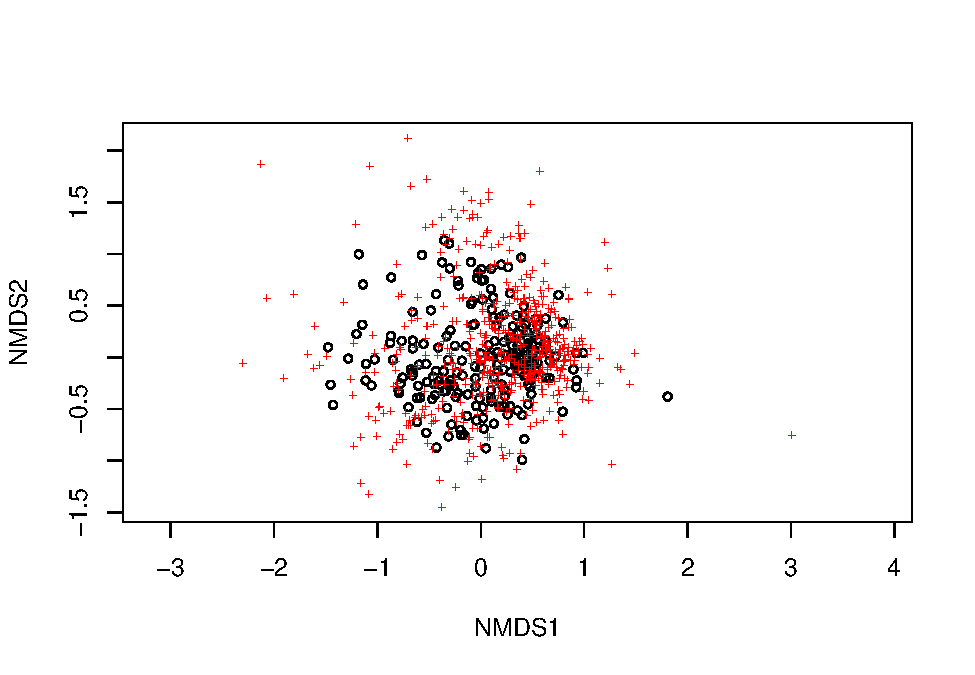
\includegraphics{bookdown-demo_files/figure-latex/unnamed-chunk-17-1.pdf}

We can adjust this using the function \texttt{display}. Play around with the code below to see how you can change the plot.

\begin{Shaded}
\begin{Highlighting}[]
\FunctionTok{plot}\NormalTok{(ordination\_spp, }\AttributeTok{display =} \StringTok{"sites"}\NormalTok{)}
\FunctionTok{text}\NormalTok{(ordination\_spp, }\AttributeTok{display =} \StringTok{"spec"}\NormalTok{, }\AttributeTok{cex =} \FloatTok{0.7}\NormalTok{, }\AttributeTok{col =} \StringTok{"blue"}\NormalTok{)}
\end{Highlighting}
\end{Shaded}

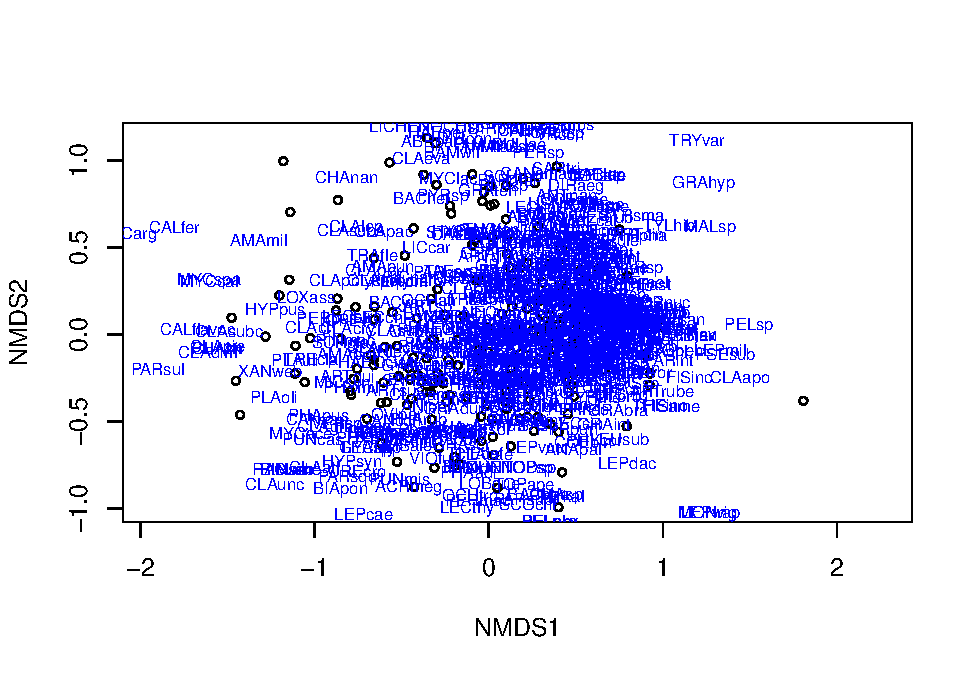
\includegraphics{bookdown-demo_files/figure-latex/unnamed-chunk-18-1.pdf}

The \texttt{text} function adds the species names. There are so many that they become illegible. You could try adjusting the font size, or if this were your own data, you might apply 2-letter species codes, if possible.

Often we want to layer other information on an ordination to better see pattern. For example, we might want to add convex hulls around the site points that are from the same ecoregion. This will let us see whether some ecoregions have species that are unique to them (the hull will be isolated from other hulls) or if two or more ecoregions have similar species composition (the hulls will have a lot of overlap).

Before we do that, we need to strip the ``sites'' column from the \texttt{MACPsites} dataframe so we have just the environmental variables. We could use the baseR method we did above to create \texttt{spp}, or you could use the \texttt{select} function from the \texttt{dplyr} package.

\begin{Shaded}
\begin{Highlighting}[]
\NormalTok{env }\OtherTok{\textless{}{-}} \FunctionTok{select}\NormalTok{(MACPsites, ER, VEG, PPT, TEMP, ELEV)}
\end{Highlighting}
\end{Shaded}

Then specify to create convex hulls using the ecoregion field (\texttt{ER}) from \texttt{env}:

\texttt{ordihull(ordination\_spp,\ env\$ER,\ col\ =\ 1:4,\ label\ =\ TRUE)}

Try the above code, and then see if you can modify it to create convex hulls by vegetation type.

If you can't see the hulls because the text labels are too big, change \texttt{label\ =\ TRUE} to \texttt{label\ =\ FALSE} and run the code again.

Another data visualization might be to use ellipses instead of convex hulls. You can try it with this code:

\texttt{ordiellipse(ordination\_spp,\ env\$ER,\ col\ =\ 1:4,\ draw\ =\ "polygon")}

Finally, we might want to do a test to see how different environmental variables at the sites load onto to the two axis of our ordination. This can start to tell us how what's happening at the sites might be influencing the species pattern(s).

\texttt{ord.fit\ \textless{}-\ envfit(ordination\_spp\ \textasciitilde{}\ ELEV\ +\ PPT\ +\ TEMP,\ data\ =\ env,\ perm\ =\ 999)}

To see the test output, type \texttt{ord.fit}

To plot the fits of elevation, temperature and precipitation on the ordination, use these to lines of code.

\texttt{plot(ordination\_spp)}
\texttt{plot(ord.fit,\ col\ =\ "black")}

\hypertarget{your-assignment-for-part-3}{%
\chapter{Your assignment for Part 3}\label{your-assignment-for-part-3}}

\begin{enumerate}
\def\labelenumi{\arabic{enumi}.}
\item
  Describe what you can conclude about the effect of latitude on species richness for the mid-Atlantic Coastal Plain. Is the fit significant? Are there issues with the data that might affect the inferences drawn from the statistical analysis?
\item
  What interpretation can you make from the final ordination plot we made here?
\item
  Think about a possible hypothesis that \citet{McMullin2019} could have tested with these data, but did not.
\end{enumerate}

\begin{itemize}
\tightlist
\item
  Write out the hypothesis in words and include a prediction
\item
  Sketch a ``toy graph'' of how you expect the data to look if the hypothesis is supported
\item
  Identify what kind of statistical test you will apply
\item
  Describe how what steps you need to take with these data to execute the steps (i.e., do you need to do any data wrangling first?). A flow chart or bullet points would be a good way to do this.
\item
  Execute the test. Include a copy of the code, the statistical output and a short interpretation of the hypothesis test.
\end{itemize}

\textbf{For graduate students}: Do the above step twice (i.e., test two different hypotheses). Challenge yourself to try a new test that you may not have done before.

  \bibliography{book.bib,packages.bib}

\end{document}
